% vim: set spell spelllang=en tw=100 et sw=4 sts=4 foldmethod=marker foldmarker={{{,}}} :

\documentclass{beamer}

\usepackage{tikz}
\usepackage{xcolor}
\usepackage{complexity}
\usepackage{hyperref}
\usepackage{microtype}
\usepackage{amsmath}                   % \operatorname
\usepackage{amsfonts}                  % \mathcal
\usepackage{amssymb}                   % \nexists
\usepackage{gnuplot-lua-tikz}          % graphs
\usepackage[vlined]{algorithm2e} % algorithms
\usepackage{centernot}
\usepackage{mathtools}
\usepackage{listings}

\usetikzlibrary{shapes, arrows, shadows, calc, positioning, fit}
\usetikzlibrary{decorations.pathreplacing, decorations.pathmorphing, shapes.misc}
\usetikzlibrary{tikzmark}

\definecolor{uofguniversityblue}{rgb}{0, 0.219608, 0.396078}

\definecolor{uofgheather}{rgb}{0.356863, 0.32549, 0.490196}
\definecolor{uofgaquamarine}{rgb}{0.603922, 0.72549, 0.678431}
\definecolor{uofgslate}{rgb}{0.309804, 0.34902, 0.380392}
\definecolor{uofgrose}{rgb}{0.823529, 0.470588, 0.709804}
\definecolor{uofgmocha}{rgb}{0.709804, 0.564706, 0.47451}
\definecolor{uofgsandstone}{rgb}{0.321569, 0.278431, 0.231373}
\definecolor{uofgforest}{rgb}{0, 0.2, 0.129412}
\definecolor{uofglawn}{rgb}{0.517647, 0.741176, 0}
\definecolor{uofgcobalt}{rgb}{0, 0.615686, 0.92549}
\definecolor{uofgturquoise}{rgb}{0, 0.709804, 0.819608}
\definecolor{uofgsunshine}{rgb}{1.0, 0.862745, 0.211765}
\definecolor{uofgpumpkin}{rgb}{1.0, 0.72549, 0.282353}
\definecolor{uofgthistle}{rgb}{0.584314, 0.070588, 0.447059}
\definecolor{uofgrust}{rgb}{0.603922, 0.227451, 0.023529}
\definecolor{uofgburgundy}{rgb}{0.490196, 0.133333, 0.223529}
\definecolor{uofgpillarbox}{rgb}{0.701961, 0.047059, 0}
\definecolor{uofglavendar}{rgb}{0.356863, 0.301961, 0.580392}

\tikzset{vertex/.style={draw, circle, inner sep=0pt, minimum size=0.5cm, font=\small\bfseries}}
\tikzset{notvertex/.style={vertex, color=white, text=black}}
\tikzset{plainvertex/.style={vertex}}
\tikzset{vertexc1/.style={vertex, fill=uofgburgundy, text=white}}
\tikzset{vertexc2/.style={vertex, fill=uofgsandstone, text=white}}
\tikzset{vertexc3/.style={vertex, fill=uofgforest, text=white}}
\tikzset{vertexc4/.style={vertex, fill=uofgheather, text=white}}
\tikzset{edge/.style={color=black!50!white}}
\tikzset{bedge/.style={ultra thick}}
\tikzset{edged/.style={color=screengrey, dashed}}
\tikzset{edgel3/.style={color=uofgrose, ultra thick}}

% {{{ theme things
\useoutertheme[footline=authortitle]{miniframes}
\useinnertheme{rectangles}

\setbeamerfont{block title}{size={}}
\setbeamerfont{title}{size=\large,series=\bfseries}
\setbeamerfont{section title}{size=\large,series=\mdseries}
\setbeamerfont{author}{size=\normalsize,series=\mdseries}
\setbeamercolor*{structure}{fg=uofguniversityblue}
\setbeamercolor*{palette primary}{use=structure,fg=black,bg=white}
\setbeamercolor*{palette secondary}{use=structure,fg=white,bg=uofgcobalt}
\setbeamercolor*{palette tertiary}{use=structure,fg=white,bg=uofguniversityblue}
\setbeamercolor*{palette quaternary}{fg=white,bg=black}

\setbeamercolor*{titlelike}{parent=palette primary}

\beamertemplatenavigationsymbolsempty

\setbeamertemplate{title page}
{
    \begin{tikzpicture}[remember picture, overlay]
        \node at (current page.north west) {
            \begin{tikzpicture}[remember picture, overlay]
                \fill [fill=uofguniversityblue, anchor=north west] (0, 0) rectangle (\paperwidth, -2.6cm);
            \end{tikzpicture}
        };

        \node (logo) [anchor=north east, shift={(-0.6cm,-0.6cm)}] at (current page.north east) {
            \includegraphics*[keepaspectratio=true,scale=0.7]{UoG_keyline.pdf}
        };

        \node [anchor=west, xshift=0.2cm] at (current page.west |- logo.west) {
            \begin{minipage}{0.65\paperwidth}\raggedright
                {\usebeamerfont{title}\usebeamercolor[white]{}\inserttitle}\\[0.1cm]
                {\usebeamerfont{author}\usebeamercolor[white]{}\insertauthor}
            \end{minipage}
        };
    \end{tikzpicture}
}

\setbeamertemplate{section page}
{
    \begin{centering}
        \begin{beamercolorbox}[sep=12pt,center]{part title}
            \usebeamerfont{section title}\insertsection\par
        \end{beamercolorbox}
    \end{centering}
}

\newcommand{\frameofframes}{/}
\newcommand{\setframeofframes}[1]{\renewcommand{\frameofframes}{#1}}

\makeatletter
\setbeamertemplate{footline}
{%
    \begin{beamercolorbox}[colsep=1.5pt]{upper separation line foot}
    \end{beamercolorbox}
    \begin{beamercolorbox}[ht=2.5ex,dp=1.125ex,%
        leftskip=.3cm,rightskip=.3cm plus1fil]{author in head/foot}%
        \leavevmode{\usebeamerfont{author in head/foot}\insertshortauthor}%
        \hfill%
        {\usebeamerfont{institute in head/foot}\usebeamercolor[fg]{institute in head/foot}\insertshortinstitute}%
    \end{beamercolorbox}%
    \begin{beamercolorbox}[ht=2.5ex,dp=1.125ex,%
        leftskip=.3cm,rightskip=.3cm plus1fil]{title in head/foot}%
        {\usebeamerfont{title in head/foot}\insertshorttitle}%
        \hfill%
        {\usebeamerfont{frame number}\usebeamercolor[fg]{frame number}\insertframenumber~\frameofframes~\inserttotalframenumber}
    \end{beamercolorbox}%
    \begin{beamercolorbox}[colsep=1.5pt]{lower separation line foot}
    \end{beamercolorbox}
}

% }}}

\title{Search and Discrepancies}
\author[Ciaran McCreesh and Patrick Prosser]{\textbf{Ciaran McCreesh} and Patrick Prosser}

\begin{document}

{
    \usebackgroundtemplate{
        \tikz[overlay, remember picture]
        \node[at=(current page.south), anchor=south, inner sep=0pt]{\includegraphics*[keepaspectratio=true, width=\paperwidth]{background2.jpg}};
    }
    \begin{frame}[plain,noframenumbering]
        \titlepage
    \end{frame}
}

\begin{frame}{This Week's Lectures}
    \begin{columns}
        \column{.6\textwidth}
        \begin{itemize}
            \item \textcolor{uofgcobalt}{Search and Discrepancies}
                \begin{itemize}
                    \item Recap of search and heuristics
                    \item Ideas and techniques
                    \item Implementation
                \end{itemize}
            \item Parallel Constraint Programming
            \item Parallel Search
        \end{itemize}
        \column{.4\textwidth}
        \centering\includegraphics*[keepaspectratio=true,scale=0.5]{search-but-not-as-we-know-it.jpg}
        \begin{center}``It's search, Jim, but not\\as we know it.''\end{center}
    \end{columns}
\end{frame}

\begin{frame}{Maintaining Arc Consistency (MAC)}
    \begin{itemize}
        \item Achieve (generalised) arc consistency (AC3, etc).
        \item If we have a domain wipeout, backtrack.
        \item If all domains have one value, we're done.
        \item Pick a variable (using a heuristic) with more than one value, then branch:
            \begin{itemize}
                \item Try giving it one of its possible values (using a heuristic), and recurse.
                \item If that failed, reject that value, pick a new value, and try again.
                \item If we run out of values, backtrack.
            \end{itemize}
    \end{itemize}
\end{frame}

\begin{frame}{Search as a Tree}

    \centering
    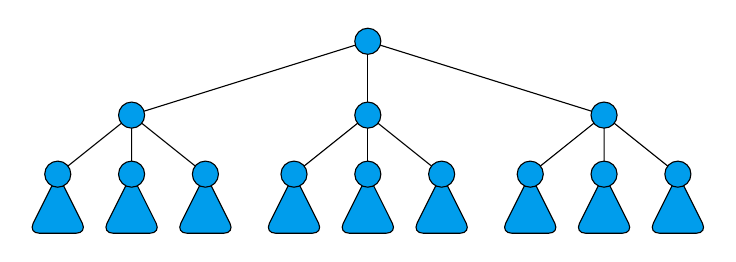
\begin{tikzpicture}[scale=0.75]%{{{
        \coordinate (R);

        \coordinate (N) at (R);

        \coordinate (N1) at ($(N) + (-4, -1.25)$);
        \coordinate (N2) at ($(N) + ( 0, -1.25)$);
        \coordinate (N3) at ($(N) + ( 4, -1.25)$);

        \foreach \na in {1, ..., 3}{
            \coordinate (N\na 1) at ($(N\na) + (-1.25, -1)$);
            \coordinate (N\na 2) at ($(N\na) + ( 0,    -1)$);
            \coordinate (N\na 3) at ($(N\na) + ( 1.25, -1)$);

            \foreach \nb in {1, ..., 3}{
                \coordinate (N\na\nb t1) at ($(N\na\nb) + (-0.5, -1)$);
                \coordinate (N\na\nb t2) at ($(N\na\nb) + ( 0.5, -1)$);
            }
        }

        \foreach \na in {1, ..., 3}{
            \draw (N) -- (N\na);
            \foreach \nb in {1, ..., 3}{
                \draw (N\na) -- (N\na\nb);
            }
        }

        \tikzstyle{t} = [draw, fill, fill=uofgcobalt, rounded corners];
        \foreach \na in {1, ..., 3}{
            \foreach \nb in {1, ..., 3}{
                \draw [t] (N\na\nb) -- (N\na\nb t1) -- (N\na\nb t2) -- cycle;
            }
        }

        \tikzstyle{c} = [draw, circle, fill, fill=uofgcobalt];
        \node [c] at (N) { };

        \foreach \na in {1, ..., 3}{
            \node [c] at (N\na) { };

            \foreach \nb in {1, ..., 3}{
                \node [c] at (N\na\nb) { };
            }
        }
    \end{tikzpicture}%}}}

    \vspace{1em}

    \begin{itemize}
        \item Circles are recursive calls, triangles are `big' subproblems.
        \item Heuristics determine the `shape' of the tree:
            \begin{itemize}
                \item Variable-ordering heuristics determine the number of children at each level.
                \item Value-ordering heuristics determine the paths explored.
            \end{itemize}
        \item MAC is like Depth-First Search (DFS).
    \end{itemize}
\end{frame}

\begin{frame}{Heuristics and Discrepancies}

    \begin{itemize}
        \item If our value-ordering heuristics are perfect, and an instance is satisfiable, we walk
            straight to a solution by going left at every level.
        \item If an instance is unsatisfiable, perfect variable-ordering heuristics would give the
            smallest possible search tree.
        \item But heuristics aren't perfect\ldots
        \item We call going against a value-ordering heuristic choice a ``discrepancy''.
    \end{itemize}

\end{frame}

\begin{frame}{Two Claims Regarding Value-Ordering Heuristics}

    \centering
    \includegraphics*[keepaspectratio=true,scale=0.3]{lds-paper.png}
    \vspace{1em}

    \begin{enumerate}
        \item The total number of discrepancies to find a solution is usually low (our
            value-ordering heuristics are \emph{usually} right).
        \item Value-ordering heuristics are most likely to wrong higher up in the tree (there is
            least information available when no or few choices have been made).
    \end{enumerate}

\end{frame}

\begin{frame}{So What?}

    \begin{itemize}
        \item If these claims are true, depth-first search is a bad idea: we're committing entirely
            to the first decision made, which is most likely to be wrong.
    \end{itemize}

\end{frame}

\begin{frame}{Limited Discrepancy Search}

    \setbeamertemplate{itemize/enumerate body begin}{\footnotesize}
    \setbeamertemplate{itemize/enumerate subbody begin}{\scriptsize}

    \begin{columns}[T]
        \column{.6\textwidth}
        \begin{itemize}
            \item First, search with no discrepancies.
            \item Then search allowing one discrepancy.
                \begin{itemize}
                    \item First try one discrepancy at the top.
                    \item Then try one discrepancy at the second level.
                    \item Then try one discrepancy at the third level.
                    \item \ldots
                \end{itemize}
            \item Then search allowing two discrepancies.
                \begin{itemize}
                    \item At the top, and at the second level.
                    \item Then at the top, and at the third level.
                    \item \ldots
                    \item Then at the second level and the third level.
                    \item \ldots
                \end{itemize}
            \item \ldots
        \end{itemize}

        \column{.4\textwidth}
        \centering\includegraphics*[keepaspectratio=true,scale=0.18]{lds-tree.png}
    \end{columns}

\end{frame}

\begin{frame}{Completeness}
    \begin{columns}
        \column{.75\textwidth}
        \begin{itemize}
            \item Complete: yes means yes, no means no.
            \item Incomplete: yes means yes, no means maybe.
            \item LDS is \emph{quasi-complete}: if the total number of discrepancies is allowed to go
                high enough, it is complete.
        \end{itemize}
        \column{.25\textwidth}
        \centering\includegraphics*[keepaspectratio=true,scale=0.4]{quasi.jpg}
    \end{columns}
\end{frame}

\begin{frame}{What About Non-Binary Trees?}
    \begin{itemize}
        \item We can rewrite our search tree to be binary. Instead of branching on each value for a
            variable in a loop, pick a variable and a value, and branch twice:

            \begin{itemize}
                \item Yes, the variable takes that value.
                \item No, the variable does not take that value.
            \end{itemize}

        \item But this means that giving the 10th value to a variable counts as 9 discrepancies. Is
            this good or bad?
    \end{itemize}
\end{frame}

\begin{frame}{Improved Limited Discrepancy Search}

    \centering\includegraphics*[keepaspectratio=true,scale=0.4]{ilds-paper.png}
    \vspace{1em}
    \begin{itemize}
        \item LDS explores some parts of the search tree more than once.
        \item Improved Limited Discrepancy Search (ILDS) does less repeated work.
    \end{itemize}

\end{frame}

\begin{frame}{Improved?}
    \begin{columns}
        \column{.5\textwidth}
        \centering\includegraphics*[keepaspectratio=true,scale=0.4]{ilds-paths.png}
        \column{.5\textwidth}
        \centering\includegraphics*[keepaspectratio=true,scale=0.18]{lds-tree.png}
    \end{columns}

\end{frame}

\begin{frame}{So is the Second Claim Important?}
    \centering\includegraphics*[keepaspectratio=true,scale=0.4]{ldsr-paper.png}

    \vspace{2em}

    \centering\includegraphics*[keepaspectratio=true,scale=0.4]{ldsr-conclusion.png}

\end{frame}

\begin{frame}{Depth-Bounded Discrepancy Search}

    \centering\includegraphics*[keepaspectratio=true,scale=0.2]{dds-paper.png}
    \vspace{1em}

    \begin{columns}[T]
        \column{.55\textwidth}
        \begin{itemize}
            \item If the second claim \emph{is} important, why not emphasise it more?

            \item Depth-bounded discrepancy search considers $k$ discrepancies, but only at depth up
                to $k - 1$ (but in which order?).
        \end{itemize}
        \column{.45\textwidth}
        \centering\includegraphics*[keepaspectratio=true,scale=0.2]{dds-tree.png}
    \end{columns}

\end{frame}

\begin{frame}{What About Unsatisfiable Instances?}

    \begin{itemize}
        \item Discrepancy searches do more total work if there is no solution.

        \item There are search variants which are better for unsatisfiable instances, and for
            optimisation problems.
    \end{itemize}

\end{frame}

\begin{frame}{Using LDS?}
    \begin{center}
        \includegraphics*[keepaspectratio=true,scale=0.2]{lds-patent.png}
    \end{center}
\end{frame}

\begin{frame}{Discrepancy Searches in Choco}

\end{frame}

\begin{frame}{Some Experiments}

\end{frame}

\begin{frame}{This is Not The Exam Question}

    What are the two assumptions regarding value ordering heuristics which underly limited
    discrepancy search? \\[0.5cm]

    Why are discrepancy searches a bad choice if instances are expected to be unsatisfiable?

\end{frame}

\begin{frame}[plain,noframenumbering]
    \begin{tikzpicture}[remember picture, overlay]
        \node at (current page.north west) {
            \begin{tikzpicture}[remember picture, overlay]
                \fill [fill=uofguniversityblue, anchor=north west] (0, 0) rectangle (\paperwidth, -1.7cm);
            \end{tikzpicture}
        };

        \node (logo) [anchor=north east, shift={(-0.3cm,-0.2cm)}] at (current page.north east) {
            \includegraphics*[keepaspectratio=true,scale=0.55]{UoG_keyline.pdf}
        };
    \end{tikzpicture}
\end{frame}

\end{document}


